%iffalse
\let\negmedspace\undefined
\let\negthickspace\undefined
\documentclass[journal,12pt,onecolumn]{IEEEtran}
\usepackage{cite}
\usepackage{amsmath,amssymb,amsfonts,amsthm}
\usepackage{algorithmic}
\usepackage{graphicx}
\usepackage{textcomp}
\usepackage{xcolor}
\usepackage{txfonts}
\usepackage{listings}
\usepackage{enumitem}
\usepackage{mathtools}
\usepackage{gensymb}
\usepackage{comment}
\usepackage[breaklinks=true]{hyperref}
\usepackage{tkz-euclide} 
\usepackage{listings}
\usepackage{gvv}                                        
%\def\inputGnumericTable{}                                 
\usepackage[latin1]{inputenc}     
\usepackage{xparse}
\usepackage{color}                                            
\usepackage{array}                                            
\usepackage{longtable}                                       
\usepackage{calc}                                             
\usepackage{multirow}
\usepackage{multicol}
\usepackage{hhline}                                           
\usepackage{ifthen}                                           
\usepackage{lscape}
\usepackage{tabularx}
\usepackage{array}
\usepackage{float}
\usepackage{tikz}           
\usetikzlibrary{patterns}
\newtheorem{theorem}{Theorem}[section]
\newtheorem{problem}{Problem}
\newtheorem{proposition}{Proposition}[section]
\newtheorem{lemma}{Lemma}[section]
\newtheorem{corollary}[theorem]{Corollary}
\newtheorem{example}{Example}[section]
\newtheorem{definition}[problem]{Definition}
\newcommand{\BEQA}{\begin{eqnarray}}
\newcommand{\EEQA}{\end{eqnarray}}
\newcommand{\define}{\stackrel{\triangle}{=}}
\theoremstyle{remark}
\newtheorem{rem}{Remark}
% Marks the beginning of the document
\begin{document}
\title{Assignment 4}
\author{EE24Btech11024 - G. Abhimanyu Koushik}
\maketitle
\renewcommand{\thefigure}{\theenumi}
\renewcommand{\thetable}{\theenumi}
\begin{enumerate}

\item The function $f\brak{t}$ satisfies the differential equation $\frac{d^2f}{dt^2}+f=0$ and the auxillary conditions, $f\brak{0}=0$, $\frac{df}{dt}\brak{0}=4$. The Laplace transform of $f\brak{t}$ is given by

\hfill{\brak{\text{ME 2013}}}
\begin{multicols}{4}
\begin{enumerate}
\item $\frac{2}{s+1}$
\item $\frac{4}{s+1}$
\item $\frac{4}{s^2+1}$
\item $\frac{2}{s^4+1}$
\end{enumerate}
\end{multicols}

\item Specific enthalpy and velocity of steam at inlet and exit of a steam turbine, running under steady state, are as given below:
\\\begin{table}[h!]    
  \centering
    \resizebox{0.7\textwidth}{!}{\begin{tabular}{l >{\centering\arraybackslash}m{3cm} >{\centering\arraybackslash}m{3cm}}
    & \underline{Specific enthalpy \brak{kJ/kg}} & \underline{Velocity \brak{m/s}} \\[5pt]
    Inlet steam condition & $3250$ & $180$ \\
    Exit steam condition & $2360$ & $5$ \\
\end{tabular}

}
\end{table}\\
The rate of heat loss from the turbine per $kg$ of steam flow rate is $5$ $kW$. Neglecting changes in potential energy of steam, the power developed in $kW$ by the steam turbine per $kg$ of the steam flow rate is

\hfill{\brak{\text{ME 2013}}}
\begin{enumerate}
\begin{multicols}{4}
\item $901.2$
\item $911.2$
\item $17072.5$
\item $17082.5$
\end{multicols}
\end{enumerate}

\item A steel ball of diameter $60$ $mm$ is initially in thermal equilibrium at $1030^\degree C$ in a furnace. It is suddenly removed from the furnace and cooled in ambient air at $30^\degree C$, with convective heat transfer coefficient $h=20$ $W/m^2K$. The thermo-physical properties of steel are: density $\rho=7800$ $kg/m^3$, conductivity $k=40$ $W/mK$ and specific heat $c=600$ $J/kgK$. The time required in seconds to cool the steel ball in air from $1030^\degree C$ to $430^\degree C$ is

\hfill{\brak{\text{ME 2013}}}
\begin{enumerate}
\begin{multicols}{4}
\item $519$
\item $931$
\item $1195$
\item $2144$
\end{multicols}
\end{enumerate}

\item A flywheel is connected to a punching machine has a supply energy of $400$ $Nm$ while running at mean angular speed of $20$ $rad/s$. If the total fluctuation of speed is not to exceed $\pm 2\%$, the mass moment inertia of the flywheel in $kg-m^2$ is

\hfill{\brak{\text{ME 2013}}}
\begin{enumerate}
\begin{multicols}{4}
\item $25$
\item $50$
\item $100$
\item $125$
\end{multicols}
\end{enumerate}

\item A compound gear train with gears $P$, $Q$, $R$ and $S$ has number of teeth $20$, $40$, $15$ and $20$, respectively. Gears $Q$ and $R$ are mounted on the same shaft as shown in the figure below. The diameter of the gear $Q$ is twice that of the gear $R$. If the module of the gear $R$ is $2$ $mm$, the centre distance in $mm$ between the gears $P$ and $S$ is
\\\begin{center}
   \scalebox{0.5}{\usetikzlibrary{patterns}
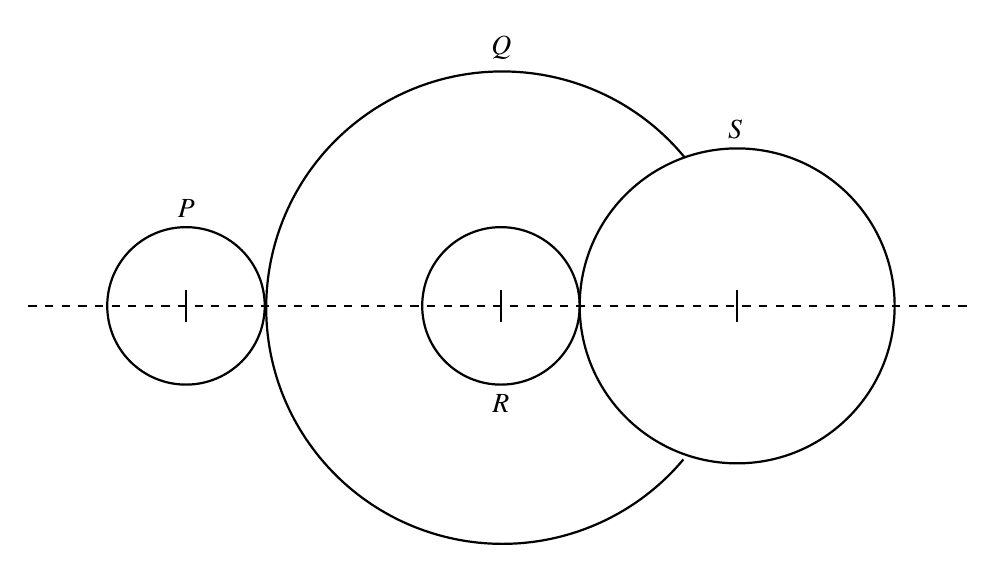
\begin{tikzpicture}
	\draw[draw=black, semithick, dashed] (-6,0) -- (6,0);
	\draw[draw=black, thick, solid] (-4,0) circle (1.00);
	\draw[draw=black, thick, solid] (2.333334,1.88563) arc[start angle=39.5, end angle=320, radius=3];
	\draw[draw=black, thick, solid] (0,0) circle (1.00);
	\draw[draw=black, thick, solid] (3,0) circle (2);
	
	\draw[draw=black, thick, solid] (-4,0.2) -- (-4,-0.2);
	\draw[draw=black, thick, solid] (0,0.2) -- (0,-0.2);
	\draw[draw=black, thick, solid] (3,0.2) -- (3,-0.2);
	
	\draw[] (-4,1) node[above] {$P$};
	\draw[] (0,-1) node[below] {$R$};
	\draw[] (0,3) node[above] {$Q$};
	\draw[] (3,2) node[above] {$S$};
\end{tikzpicture}
}
\end{center}

\hfill{\brak{\text{ME 2013}}}
\begin{enumerate}
\begin{multicols}{4}
\item $40$
\item $80$
\item $120$
\item $160$
\end{multicols}
\end{enumerate}

\item A pin jointed uniform rigid rod of weight $W$ and length $L$ is supported horizontally by an external force $F$ as shown in the figure below. The force $F$ is suddenly removed. At the instant of force removal, the magnitude of vertical reaction developed at the support is
\\\begin{center}
   \scalebox{0.5}{\usetikzlibrary{patterns}
\begin{tikzpicture}

    \draw[thick] (0,0) node[above] {$A$} -- (16,0) node[above right] {$C$} ;
    \draw[thick] (8,2.5) -- (16,2.5);

    \draw[thick] (0,0) -- (-0.8,-1) -- (0.8,-1) -- (0,0);
    \draw[thick] (-0.8,-1) -- (-1.6,-1.8);
    \draw[thick] (0,-1) -- (-0.8,-1.8);
    \draw[thick] (0.8,-1) -- (0,-1.8);
    
    \draw[dashed] (0,0) -- (0,-5);
    \draw[dashed] (8,0) node[above left] {$B$} -- (8,-5);
    \draw[dashed] (16,0) -- (16,-5);
    
    \draw[thick] (16,0) -- (15.2,-0.6) -- (16.8,-0.6) -- (16,0);
    \draw[thick] (15.6,-0.8) circle (0.2);
    \draw[thick] (16.4,-0.8) circle (0.2);
    
    \draw[thick] (15.2,-1) -- (16.8,-1);
    \draw[thick] (15.2,-1) -- (14.4,-1.8);
    \draw[thick] (16,-1) -- (15.2,-1.8);
    \draw[thick] (16.8,-1) -- (16,-1.8);
    
    \draw[->] (4,-5) node[above, font=\Large] {$2000$} -- (0,-5);
    \draw[->] (4,-5) -- (8,-5);
    \draw[->] (12,-5) node[above, font=\Large] {$2000$} -- (16,-5);
    \draw[->] (12,-5) -- (8,-5);
    
    \draw[->] (8,2.5) -- (8,0);
    \draw[->] (9,2.5) -- (9,0);
    \draw[->] (10,2.5) -- (10,0);
    \draw[->] (11,2.5) -- (11,0);
    \draw[->] (12,2.5) node[above, font=\Large] {$3000$ $Nm^{-1}$}-- (12,0);
    \draw[->] (13,2.5) -- (13,0);
    \draw[->] (14,2.5) -- (14,0);
    \draw[->] (15,2.5) -- (15,0);
    \draw[->] (16,2.5) -- (16,0);

\end{tikzpicture}
}
\end{center}

\hfill{\brak{\text{ME 2013}}}
\begin{enumerate}
\begin{multicols}{4}
\item zero
\item $\frac{W}{4}$
\item $\frac{W}{2}$
\item $W$
\end{multicols}
\end{enumerate}

\item Two cutting tools are being compared for a machine operation. The tool life equations are:
\\\begin{table}[h!]    
  \centering
  \resizebox{0.3\textwidth}{!}{\begin{tabular}{rl}
        Carbide tool: & $VT^{1.6}=3000$ \\
        HSS tool: & $VT^{0.6}=200$ \\
    \end{tabular}
}
\end{table}\\
where $V$ is the cutting speed in $m/min$ and T is the tool life in $min$. The carbide tool will provide higher tool life if the cutting speed in $m/min$ exceeds 

\hfill{\brak{\text{ME 2013}}}
\begin{enumerate}
\begin{multicols}{4}
\item $15.0$
\item $39.4$
\item $49.3$
\item $60.0$
\end{multicols}
\end{enumerate}

\item In a CAD package, mirror image of a 2D point $\vec{P}\brak{5,10}$ is to be obtained about a line which passes through origin and makes an angle $45^\degree$ counterclockwise with the X-axis. The coordinates of transformed point will be

\hfill{\brak{\text{ME 2013}}}
\begin{enumerate}
\begin{multicols}{4}
\item $\brak{7.5,5}$
\item $\brak{10,5}$
\item $\brak{7.5,-5}$
\item $\brak{10,-5}$
\end{multicols}
\end{enumerate}

\item A linear programming problem is shown below.
\\\begin{table}[h!]    
  \centering
  \resizebox{0.3\textwidth}{!}{\begin{tabular}[12pt]{ |c|c|c|}
    \hline
    \textbf{Job} & \textbf{Processing time \brak{\textbf{in days}}} & \textbf{Due Date } \\
    \hline
    $1$ & $4$ & $6$\\
    \hline 
    $2$ & $7$ & $9$\\
    \hline
    $3$ & $2$ & $19$\\
    \hline
    $4$ & $8$ & $17$\\
    \hline
\end{tabular}
}
\end{table}\\
It has

\hfill{\brak{\text{ME 2013}}}
\begin{enumerate}
\begin{multicols}{2}
\item an unbounded objective function.
\item exactly one optimal solution.
\item exactly two optimal solutions.
\item infinitely many optimal solutions.
\end{multicols}
\end{enumerate}

\item Cylindrical pins of $25^{\substack{+0.020\\+0.010}}$ $mm$ diameter are electroplated in a shop. Thickness of the plate is $30^{\pm 2.0}$ $micron$. Neglecting gauge tolerances, the size of the GO gauge in $mm$ to inspect the plated components is 

\hfill{\brak{\text{ME 2013}}}
\begin{enumerate}
\begin{multicols}{4}
\item $25.042$
\item $25.052$
\item $25.074$
\item $25.084$
\end{multicols}
\end{enumerate}

\item During the electrochemical machining \brak{\text{ECM}} of iron \brak{\text{atomic weight}=56\text{, valency}=2} at current $1000$ $A$ with $90\%$ current efficiency, the material removal rate was observed to be $0.26$ $gm/s$. If the Titanium \brak{\text{atomic weight}=48\text{, valency}=3} is machined by ECM process at the current of $2000$ $A$ with $90\%$ current efficiency, the expected material removal rate in $gm/s$ will be

\hfill{\brak{\text{ME 2013}}}
\begin{enumerate}
\begin{multicols}{4}
\item $0.11$
\item $0.23$
\item $0.30$
\item $0.52$
\end{multicols}
\end{enumerate}

\item A single degree of freedom system having mass $1$ $kg$ and stiffness $10$ $kN/m$ initially at rest is subjected to an impulse force of magnitude $5$ $kN$ for $10^{-4}$ $seconds$. The amplitude in $mm$ if the resulting free vibration is

\hfill{\brak{\text{ME 2013}}}
\begin{enumerate}
\begin{multicols}{4}
\item $0.5$
\item $1.0$
\item $5.0$
\item $10.0$
\end{multicols}
\end{enumerate}

\end{enumerate}
\end{document}

